\documentclass[11pt, english]{article}
        \usepackage{geometry}
                \geometry{
                        a4paper,total={210mm,297mm},
                        tmargin=40.8mm,
                        bmargin=40.8mm,
                        lmargin=32.6mm,
                        rmargin=32.6mm,
                }

	\usepackage{titlesec}
                \titleformat{\section}
                        {\normalfont\fontsize{18}{16}\bfseries}{\thesection}{0.5em}{}
                \titleformat{\subsection}
                        {\normalfont\fontsize{14}{16}\bfseries}{\thesubsection}{1em}{}
                \titleformat{\subsubsection}
                        {\normalfont\fontsize{11}{16}\bfseries}{\thesubsubsection}{1em}{}

	\usepackage{float}

	\usepackage{longtable}
	\usepackage{multicol}
        \usepackage{multirow}

	\usepackage{caption}
                \captionsetup[table]{labelfont=bf,textfont=bf,font=small,skip=8pt}
                \captionsetup[figure]{labelfont=bf,textfont=bf,font=small,skip=8pt}
        \usepackage{subcaption}
                \captionsetup[subtable]{labelfont=rm,textfont=rm,font=small,skip=8pt,labelformat=parens,labelsep=space}
                \captionsetup[subfigure]{labelfont=rm,textfont=rm,font=small,skip=8pt,labelformat=parens,labelsep=space}

	\renewcommand{\thetable}
                {\thesection.\arabic{table}}                                                         
	\renewcommand{\thesubtable}
                {\roman{subtable}}

	\renewcommand{\thefigure}
                {\thesection.\arabic{figure}}
        \renewcommand{\thesubfigure}
                {\roman{subfigure}}

        \usepackage{hyperref}
                \hypersetup{
                        colorlinks=true,
                        linkcolor=black,
                        filecolor=magenta,
                        urlcolor=cyan,
                        }

        \setlength{\parindent}{0pt}
        \renewcommand{\baselinestretch}{1.25}
        \usepackage{setspace}

        \usepackage{amsmath}
        \usepackage{amssymb}

	\usepackage{graphicx}

	\usepackage[utf8]{inputenc}
	\usepackage[T1]{fontenc}

\begin{document}

\pagenumbering{gobble}

	\title{\textsc{CS990 Database Fundamentals\\ Coursework Assignment}}
	\author{\textsc{Lewis Britton}}
	\date{\textsc{Academic Year 2021/2022}}
        \maketitle

\newpage

\pagenumbering{roman}

	\renewcommand{\contentsname}{Table of Contents}

	\tableofcontents

\newpage

\pagenumbering{arabic}

\section*{The Task}

	\subsection*{Requirements}

	\begin{itemize}
	\setlength\itemsep{0cm}
		\item List \textbf{entities} w/ description
		\item List \textbf{attributes} w/ \underline{underlined} \textbf{identifier}
		\item List \textbf{relationships}, for each:
		\begin{itemize}
			\item Relationship name
			\item Names of entities related
			\item Degree of relationship
			\item Optionality of relationship
		\end{itemize}
		\item List \textbf{assumptions}
		\item Enhanced Entity Relationship Diagram
	\end{itemize}

\newpage

	\subsection*{Scenario Key Words \& Phrases}

	\begin{itemize}
        \setlength\itemsep{0cm}
		\item `An' \textit{in-patient}
		\item `A' \textit{hospital}
		\item `A' \textit{patient record number}
		\item `Detail\textbf{s} of' \textit{his/her} (person), \textit{name}, \textit{address}, \textit{DoB}, \textit{allocated GP}
		\item `Patients are assigned to a single' \textit{ward}
		\item `Each ward identified by' \textit{ward number}, \textit{name}
		\item `Some wards may have 0 patients assigned to them'
		\item `Each ward staffed by \textbf{at least} one' \textit{nurse}
		\item `In a ward, a designated nurse is in charge of the ward and other nurses'
	\end{itemize}

	\begin{itemize}
        \setlength\itemsep{0cm}
		\item `Every patient allocated one' \textit{consultant}
		\item `Each consultant has recorded' \textit{specialization}
		\item `And leads team of' \textit{junior doctors}
		\item `Who may be' \textit{registrars} `or' \textit{housemen}
		\item `All' \textit{doctors} (both consultant and junior)
		\item `Have' \textit{staff numbers}, \textit{names}
		\item \textit{Teams} identified by' \textit{team code}, \textit{N. doctor members}
	\end{itemize}

	\begin{itemize}
        \setlength\itemsep{0cm}
		\item `Doctors may treat many patients'
		\item `Each patient may be treated by many doctors, always members of same team as consultant responsible for patient'
		\item `One or more' \textit{drugs} `are prescribed to patient'
		\item `Drugs identified by' \textit{name}, \textit{code number}
		\item `Also have' \textit{date}, \textit{dosage}, \textit{prescribing doctor} `for each'
		\item `Only doctors prescribe drugs'
	\end{itemize}

\newpage

\section{Preliminaries}

	\subsection{Entities \& Attributes}

	\begin{center}
		\scriptsize
		\renewcommand{\arraystretch}{1.25}
	\begin{longtable}{lp{5cm}p{4cm}}
		\textsc{Entities} & \textsc{Description} & \textsc{Attributes \& Identifiers}\\
		\hline
		\hline
		In-Patient & A patient treated in only one ward of a hospital & \underline{Patient Record No.}\newline Gender (? `His/her')\newline Name\newline Address\newline DoB\newline Allocated GP\newline Ward\\
		\hline
		Hospital & An institution in which patients are treated in asscoiated wards, doctors (consultant, junior (reg., house.)) and nurses are employed to treat and survey patients and prescribe drugs etc. & N/A\\
		\hline
		Ward & A segment of a hospital to which patients are assigned and treated in & \underline{Ward No.}\newline Name\\
		\hline
		Nurse & An employee of a hospital who staffs wards and leads other nurses & \underline{Staff No.}$^{2}$\\
		\hline
		Consultant (Doctor) & A superior (Tier 1) employee of a hosptital who consults patients, has a specialization and leads a team of junior doctors & \underline{Staff No.}\newline Name\\
		\hline
		Team & A collection of junior doctors lead by a consultant & \underline{Team Code}\newline N. Doctor Members\\
		\hline
		Junior Doctor (Doctor) & An inferior (Tier 1) employee of a hospital who is either a \textit{registrar} or a \textit{houseman} (with identical \textbf{attributes}) and is part of a team lead by a consultant, many of which may treat a patient if they are in the same consulatnt's team & \underline{Staff No.}\newline Name\\
		\hline
		Drug & An item prescribed to in-patients by only doctors, not nurses, to attempt to provide aid to in-patients & \underline{Drug Code}\newline Name\newline Date\newline Dosage\newline Prescribing Doctor\\
		\hline
		\hline
		Nurse Leader$^{1}$ & The leader of a set of nurses and the associated ward if the ward has more than one nurse. Simplifies relationship between nurses and wards & \underline{Staff No.}$^{2}$\\
		\hline
		Prescription$^{1}$ & An item used to assign drugs to patients and simplify the relationship between teams of junior doctors and drugs, and consultants and drugs. & \underline{Prescription Code}\\
		\hline
		\hline
		\multicolumn{3}{l}{$^{1}$: New Entity for Relationship}\\
		\multicolumn{3}{l}{$^{2}$: Surrogate Key}\\
		\hline
		\caption{Entities \& Attributes}
	\end{longtable}
	\end{center}

\newpage

	\subsection{Relationships}

	\begin{table}[h]
                \scriptsize
                \renewcommand{\arraystretch}{1.25}
        \begin{center}
	\begin{tabular}{lp{6cm}ll}
		\textsc{Relationship} & \textsc{Entities} & \textsc{Degree} & \textsc{Optionality}\\
		\hline
		Has & Hospital : Ward & 1:N & Obligatory\\
		Has & Ward : In-Patient & 1:N & Non-Obligatory\\
		Leads & Nurse Leader : Ward & 1:1 & Obligatory\\
		Staffs & Nurse : Ward & 1:N & Non-Obligatory\\
		Leads & Nurse Leader : Nurse & 1:N & Non-Obligatory\\
		Is Assigned To & Consultant : In-Patient & 1:N & Non-Obligatory\\
		Treats & Team : In-Patient & 1:N & Non-Obligatory\\
		Leads & Consultant : Team & 1:1 & Obligatory\\
		Contains & Team : Junior Doctor \textit{(Reg./House.)} & 1:N & Obligatory\\ 
		Is Prescribed & In-Patient : Prescription & 1:1 & Obligatory\\
		Prescribes & Consultant : Prescription & 1:N & Non-Obligatory\\
		Prescribes & Team : Prescription & 1:N & Non-Obligatory\\
		Contains & Prescription : Drug & N:M & Obligatory\\	
		\hline
	\end{tabular}
		\caption{Relationships}
	\end{center}
	\end{table}

		\subsubsection{Commentary}

	\begin{itemize}
	\setlength\itemsep{0cm}
		\item A hospital must have many wards
		\item A ward may have many in patients but may also have as little as 0
		\item A nurse leader heads a ward
		\item Nurses staff wards but 0 nurses technically may staff a ward as if there is just 1, it is a `nurse leader', not a `nurse'
		\item A nurse leader leads other nurses however, may lead 0 if it's just them on the ward
		\item A consultant is assigned to an in-patient meaning every in patient must have a consultant but some consultants may not have an in-patient. Some may have many
		\item A team (of junior doctors) is assigned to an inpatient meaning every in-patient must have a team (only treated by junior doctors from that team), but perhaps not every team is assigned in-patients, so may have 0
		\item A consultant leads one team
		\item Each team must contain a set of junior doctors
		\item Each in-patient is prescribed a prescription
		\item A consultant may prescribe many prescriptions if they have many patients, but they may also prescribe 0
		\item A team may prescribe many prescriptions if they have many patients, but they may also prescribe 0
		\item Each prescription contains one or more drugs and each drug may appear in many different prescriptions, however some may not appear in any prescriptions
	\end{itemize}

\newpage

	\subsection{Assumptions \& Explanations}

	\begin{itemize}
	\setlength\itemsep{0cm}
		\item Consultants and Junior Doctors are both \textit{Doctors} however, have different \textbf{attributes} and are therefore listed as separate \textbf{entities}
		\item Resistrars and Housemen are both \textit{Junior Doctors} however, have identical \textit{attributes} and are therefore listed as the same \textbf{entity}
		\item All wards may have no patients in a perfectly healthy world. However, for this example it is stated that at least some wards are populated, making the relationship non-obligatory
		\item There are enough nurses for at least one-per-ward
		\item If a ward is only staffed by one nurse, they may still be considered the `leader' of the ward however, they lead no other nurses making the Nurse : Nurse relathionship non-obligatory
		\item There may not be enough patients for all the consultants to be assigned to one, making the relationship non-obligatory;
		\item Therefore, if a consultant isnt assigned a patient, as teams can only treat patients associated with their consultant, some junior doctors may treat no patients, making the relationship non-obligatory
		\item As patients can be assigned a minimum of one drug by a doctor, this may either be by a consultant or a junior doctor, making each respective relationship with drug non-obligatory
		\item There are enough junior doctors in the hospital for every consultant to be lead a team
	\end{itemize}

\newpage

\section{Enhanced Entity Relationship Model (EERM)}

	\vspace{\fill}

	\begin{center}
		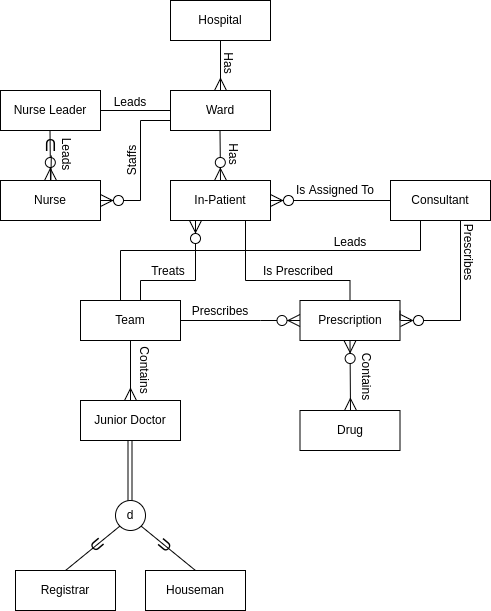
\includegraphics[height=14cm,width=12cm]{CS990_IMG/ER.png}
	\end{center}

	\vspace{\fill}

\end{document}
